\chapter{Data fusion in the Kalman module}
\section{Initial Matlab Parameter Simulation}
Before starting development for the robot, the beginning of the project was spent on building a simple \textsc{Matlab} simulation of a Kalman Filter.
This allowed the group to get acquainted to the different parameters of a Kalman Filter and to learn how they influence estimation.

By inserting velocity data and analyzing the predictions we gained much insight into the Kalman Filter model. Additionally the effects of the noise covariances became much clearer in a way that was very helpful throughout the project.

\section{ROS Package Dependencies}
\subsection{Robot localization}
For the functionality of the Kalman Filter the package \texttt{robot\_localization} is used. The package provides a convenient 15-dimensional implementation of the Kalman Filter with direct support for 6D pose, 6D velocity and 3D acceleration vectors. The available inputs can be dynamically configured in the \texttt{.launch} file for the \texttt{robot\_localization} node. In general the whole package is configurable via \texttt{.launch} file or \texttt{.yaml} file.

\subsection{TF (Transformation)}
The \texttt{TF} package is used to define all sorts of data transformations in different coordinate systems. In this case the robot's map data and the input of the marker detection are converted to be fused in a common coordinate system. 

\section{Package Structure / Design}
The Kalman package consists of three sub-packages two of which are used for development purposes. They are described in detail in the following sections:
\begin{description}
\item[\texttt{sensor\_dummy:}] Placeholder nodes used to generate artificial sensor data.
\item[\texttt{kalman\_debug:}] A package for visual monitoring and evaluation.
\item[\texttt{kalman\_global:}] The production package that performs input conversions and publishes estimates.
\end{description}

The package is designed to be highly dynamic. All properties and settings can be configured by \texttt{.yaml} files and \texttt{.launch} files similar to the \texttt{robot\_localization} package. So no recompilation is required if new topic names are chosen or the resulting frames of the data change.

\subsection{package \texttt{kalman\_global}}
This package contains the actual logic for data fusion.

For full flexibility it defines namespaces for \texttt{yaml} configurable names. For example the \texttt{node} namespace contains names for following nodes:
\begin{description}
\item[Converter] Node for converting poses into appropriate frames.
\item[EKF launch] 
\item[Launcher]
\item[Set pose]
\item[TF setup] This node broadcasts transform messages for testing purposes.
\item[Visualizer] the visual monitoring and debugging node using rviz.
\end{description}

Several IDs are listed in the \texttt{param} namespace:
\begin{description}
\item[World ID]
\item[Map ID]
\item[Odom ID]
\item[Frame ID]
\item[Base Link ID]
\end{description}

It also contains all service as well as topic names that the package listens on or publishes to:

\begin{description}
\item[Kinect topic] Derived poses from the Kinect arrive here.
\item[Laser topic] The converter listens on this topic to receive poses from laser sensors. 
\item[Laser processed topic] The laser pose is converted to the same frame as the Kinect frame and re-published here.
\item[Result topic] publishes the filtered odometry data
\item[Converted result topic] After the filtered data is converted to the frame ID it is re-published here.
\item[Is kidnapped topic] The high level module publishes a flag on this topic whenever the kidnapping state changes.
\item[Reset service] Whenever the robot has recovered from kidnapped state this service optionally allows to reset the position to the re-localized one. The feature is currently disabled for a simpler mechanism, see TODO.
\end{description}

\subsection{Robot Localization Node}
This node is a part of the \texttt{robot\_localization} package and implements the Extended Kalman Filter. It receives input from the topics of the Vision module INSERT NAME, the robot's map system and a third topic generated by the Kalman converter node in case the robot is kidnapped to prevent the continuous detection of kidnappings due to jumping output values.

\subsection{Converter Node}
The converter node handles the output of the \texttt{robot\_localization} node and republishes the data to the final topic INSERT NAME, the other modules are working with. This interception is used to filter all results of the robot's map data and only rely on camera data as long as the robot is in kidnapped state.

Moreover in case of a kidnapping the converter node publishes the camera results with reduced covariance as a third input topic to the Kalman Filter, to convince it that the camera data now has the only valid results. This is needed since the ranges of covariances between the different input topics vary vastly.

\subsection{package \texttt{sensor\_dummy}}
In the first months of the project it impossible to test the implementation with real input since all teams started from scratch. Production and publication of sensor data was just being developed. To overcome this obstacle artificial test data was generated and used as output of placeholder sensor nodes. 

Test data from two different generation techniques have been employed: a quick but very unrealistic solution in \textsc{Matlab} and later a more sophisticated simulation using the MonoGame framework.

\subsection{Test data from \textsc{Matlab}}
In \textsc{Matlab} test data was generated by supplying a number of points provided by the user and distributed over time. The \textsc{Matlab} script uses a cubic spline interpolation to generate the values in between. For simplicity these values were initially only generated for one dimension of the Kalman Filter.

Primitive testing was possible with this data virtually from day one.

\subsection{Simple MonoGame}
For the generation of more realistic testdata, including 2D poses and robot view angle, a small \texttt{C\#}-program was built. This program uses the MonoGame framework to allow mouse interaction in a window. A small arrow is displayed to represent the robot. Then by clicking on a position the user can tell the robot to move there with a pre-defined fixed speed. When holding down the mouse button and releasing it on another pixel the vector between these points is used to generate the target view angle of the robot. In the background the program continuously writes the current position and view angle to a file.

\subsection{Sensor Test Data Dummy node}
Two placeholder sensor nodes -- representing laser sensor and Kinect -- read from the test data files and published them in a loop as \texttt{PoseWithCovarianceStamped} and \texttt{Twist}. This way the Kalman Filter could be tested even if the actual sensor nodes were still in development. It was now possible to tweak the many parameters of the \texttt{robot\_localization node} and study the filters behavior independently of the other groups.

\subsection{Rviz Simulation}
After development of the input and procesing pipeline for test data, the next challenge was to evaluate the filter's outputs. Since humans are very ineffective in classifying text data, the ROS package \texttt{rviz} was utilized to visually compare input data and filtered result. The visual proof for the effects of parameter changes greatly enhanced our capability to evaluate the Kalman filter's performance. In the figures \ref{Fig: Kalman Fusion - Low}, \ref{Fig: Kalman Fusion - Medium} and \ref{Fig: Kalman Fusion - High} the behaviour of the X-Component of the Target Position is visualized. The blue line represents the position received from the Vision Group. While the red line represents the data received from the robots mapping module. The green line is the fused data of the kalman filter. The jumps to the blue value are triggered by the Highlevel Group when a kidnapped signal is received. Depending on the system's confidence the jump back to normal has different speeds.

\begin{figure}[thpb]
      \centering
      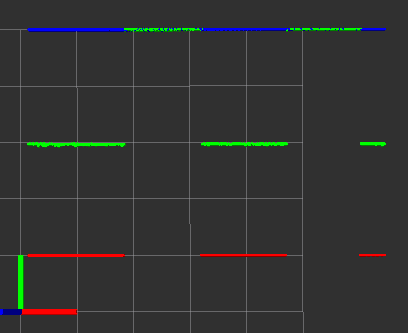
\includegraphics[width=0.5\textwidth]{graphics/kalman_fast.png}
      %\includegraphics[scale=1.0]{figurefile}
      \caption{Kalman fusion - Low System Confidence}
      \label{Fig: Kalman Fusion - Low}
   \end{figure}

\begin{figure}[thpb]
      \centering
      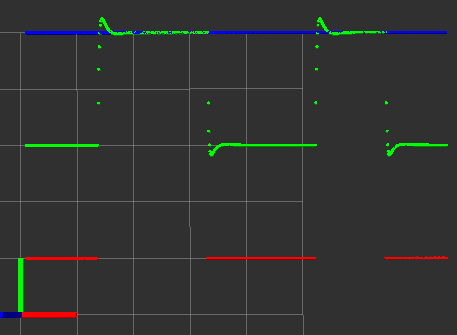
\includegraphics[width=0.5\textwidth]{graphics/kalman_medium.png}
      %\includegraphics[scale=1.0]{figurefile}
      \caption{Kalman fusion - Medium System Confidence}
      \label{Fig: Kalman Fusion - Medium}
   \end{figure}
	
\begin{figure}[thpb]
      \centering
      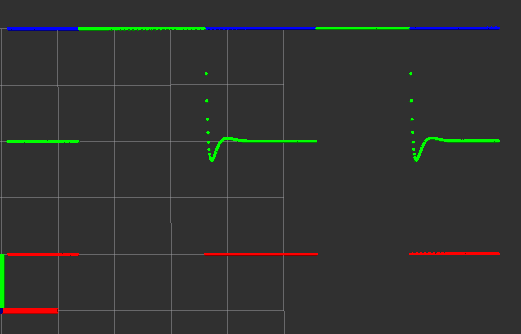
\includegraphics[width=0.5\textwidth]{graphics/kalman_slow.png}
      %\includegraphics[scale=1.0]{figurefile}
      \caption{Kalman fusion - High System Confidence}
      \label{Fig: Kalman Fusion - High}
   \end{figure}

\subsection{visualization node}
The visualization node subscribes to the output topic of the Kalman Filter and the input topcis from the robot to create displayable data which can be used to verify the data fusion quality. This displayable data are markers published to \texttt{rviz} that shows them in its coordinate system. There are two possible visualization modes:

\begin{itemize}
\item Show the current 2D Pose of the robot
\item Show timely change of the robot's pose in x.
\end{itemize}

It is also possible to display process covariances over time to gain a better understanding of why there might be a sudden change in the kalman filter's behaviour.

\section{Difficulties}
\subsection{Initial start with custom Kalman Implementation}
Before using the \texttt{robot\_localization} package a quick attempt to implement the Kalman Filter manually was investigated. Luckily our attention was directed towards the \texttt{robot\_localization} package before more than data subscription and publishing were implemented, both of which were fortunately reused throughout the project.

\subsection{Difficulties with employing MCA2}
When the Kalman Filter performed satisfactorily with the artificial test data, the next step consisted of producing more realistic data with a true robot simulator. For this MCA2 appeared to be a suitable solution. But the installation of MCA2 and the simulator presented unexpected difficulties and failed in the end.

One of the reasons is the quality of the MCA2 documentation which posed a major problem. It is highly fragmented, redundant, often outdated and in some places contradictory. Very often it was difficult to understand if an installation error was caused by a user mistake or by the documentation and if the latter, whether it is only unclear, incomplete or incorrect. 

The usual approach for a computer scientist is to read the documentation and rule out any self-made errors before asking possibly unnecessary questions. This is why the lacking documentation caused more harm than good.

It was finally discovered that additional data only existing on a USB drive was required in order for the package to install successfully. But even after having received this piece of data the software could only be run exclusively on lab computers, indicating another still unknown dependency or requirement.

By that time data publishing and necessary software for it have already been facilitated on the robot. So MCA2 was abandoned and the robot itself was used to generate data.

\subsection{Roslaunch initialization and ROS\_IP behind NATs}
While working with virtual machines for ROS package development the problem of incorrect communication between the packages was discovered. Only when starting the nodes in the right order with appropriate delays in between, the system would work on the robot. In general the specification of the \texttt{ROS\_IP} environment variable is used to solve that issue. The local IP of the virtual machines behind a NAT was not available and so the execution of the nodes was completely moved to the robot.

\subsection{Wifi Overload $\Rightarrow$ huge delays}
When attaching the camera to the robot in a manner that the image data has to be sent over wifi, the whole ROS communication is extremly slow. This problem is solved by installing all drivers for the camera on the robot. So the camera and its related nodes can operate locally on the robot.

\subsection{Boundary for accepted jumps between sensor outputs}
When first configuring the \texttt{robot\_localization} package, a threshold for tolerated jumps in the sensor data was set to a rather low value. This caused the Kalman Filter to exhibit a lot of unexpected behavior, for instance it did not respect changes in one sensor at all. After setting the threshold to an appropriate value, the filter worked even better as initially expected. This is partly due to the well adjusted remaining parameters of the Kalman Filter which were already thoroughly tested with the Matlab simulation.

\subsection{Set pose of robot\_localization does not work as expected}
The \texttt{robot\_localization} package provides a \texttt{set\_pose} topic to force the actual pose of the robot. It was planned to use this topic to inform the Kalman Filter about the new pose after having recovered the robot from kidnapped state. Unfortunately this sets the pose permanently and further input is ignored, so another solution was necessary.

The approach of choice uses a third virtual input sensor that sends the recovered pose along with very low covariances to convince the Kalman Filter to trust this source the most.

But in the final implementation the necessity to react to a kidnap event was disabled in the Kalman filter. Instead, we opted for a simpler behaviour: the high level logic updates the transform immediately after having resolved the kidnapping, so that sensor data discrepancies are removed. 

\subsection{Unclear information about the data source topics and types for the data fusion}
Finding out which scripts must be started on the robot to make it publish its pose and twist turned out to be a challenge in itself. During some periods alternative topics were used to at least receive any data to work with. For example the map position of the robot was temporarily replaced by its odometry output.